\section{Grace Hopper}

While Grace Hopper may not have been the first
to create a program that punched
out another program as its output, she pioneered the field of compilation to the
extent that many consider her the inventor of compilers.Her innovations were
also more readily adopted than those at the ETH.Consider Figure
\ref{fig:dawn-timeline}, and the pace of development in Hopper's time compared
to the years prior.Note that while we have ample data on \textit{how} Hopper's
compiler worked and how she and her team developed it, the intuition behind
those developments is foggy at best. We have recollections from Hopper and her
contemporaries, but only from long after the fact. It was not understood at the
time how important her work was, so we have only to speculate and piece together
oral histories.

Originally a mathematics professor at Vassar College, Hopper
obtained waivers for her age and weight and joined the U.S. Navy in 1943,
eventually graduating first in her class from Midshipmen's School. She was
assigned, somewhat unexpectedly, to Commander Howard Aiken's Harvard
Computation Laboratory in 1944as the third programmer of the Automatic Sequence
Controlled Calculator (Mark I), the world's first operational computer. Although
it was significantly slower than the ENIAC, it was \textit{programmable}; the
ENIAC had to be physically rewired to change its program. To write a compiler
for the ENIAC, one would need to plug the phone lines in the back of the
machine together to create the compiler, feed in the input program as data, and
a human operator would have to take the punchcards it produced and manually
rewire the machine to run that program.

Aiken built the Mark I in collaboration
with IBM, though it is unclear how much either side contributed in its
development. The proportion of credit given to either party would be disputed in
numerous documents and press releases in the following years, including
the \textit{Manual of Operation for the Automatic Sequence Controlled
	Calculator}, the technical manual for the Mark I. In the fall of 1944, Aiken
decided that his team needed to produce a book documenting the
technical developments at the Harvard Computation Laboratory and how the Mark I
was intended to be used. For this task, he chose Hopper; though she protested,
her reputation as a clear and thoughtful communicator and writer had already
earned her the job. Hopper was known for her writing ability, and it was a point
of emphasis in her teaching career. She would assign her mathematics students
onerous writing tasks to emphasize that "it was no use trying to learn math
unless they could communicate with other people."
\cite[interview on 5 July, 1972]{grace_hopper_and_the_invention_of_the_information_age_2009}

Aiken and Hopper both understood that, for the Mark I to be a success, it would be used
and understood by a large and diverse audience, and for that to happen, they
needed a detailed, compelling, and accessible
manual.\cite{annals_of_the_computation_laboratory_of_harvard_university_1946}:

% \todo{% ENIAC, could not be programmed (had to be rewired to be
% programmed)% but was real fast. Aiken's Mark I.% Fall 1944, Aiken
% wants to record technical developments at Harvard Computation
% Laboratory (as book), % chose Hopper, to her disagreement. Finished
% 561 page manuscript, published 1946.% She believed she was chosen
% for "clear, fluid prose."% her time as a math teacher made her good
% at writing/explaining things.% would force students to write essays
% on math topics and would grade harshely.% "it was no use trying to
% learn math unless they could communicate with other people."% Aiken
% and Hopper knew a large/diverse audience would need to understand
% it for it to% be successful; high value on good
% writing+communication.% Aiken's strict heirarchy+meritocracy
% allowed her to compete with the men.% IBM tried to steal all the
% credit for the Mark I from Aiken.% aiken distaste for being
% assigned woman officer, but meritocracy.% }

\subsection{Hopper and the Mark I's Manual}

Here we drift into some general computing history,
mostly because it was so formative for Hopper, who was in turn so
formative in the development of compilers.
Her manual for the Mark I
began with a detailed and dramatic retelling of computing history,
opening with the following quote from Charles Babbage
and culminating with the Mark I:

\begin{quotation}
	If, unwarned by my example, any man shall undertake
	and shall succeed in really constructing an engine embodying in
	itself the whole of the executive department of mathematical
	analysis upon different principles or by simpler mechanical means, I
	have no fear of leaving my reputation in his charge, for he alone
	will be fully able to appreciate the nature of my efforts and the
	value of their results.
\end{quotation}

Her history went on to cover:
\begin{itemize}
	\item Blaise Pascal's counting machines, "foundation on which
	      nearly all mechanical
	      calculating machines since have been constructed."
	\item Leibniz; stepped wheels system for mul/divs.
	\item Charles Babbage; most significant part of the manual dedicated to him.
	      Difference engine, idea for computing machine. Invented punch card system to
	      feed in information, made after textile looms. G H emphasized the
	      machine would
	      take 2 decks of cards, one for data, one for instructions (not
	      von neumann).
	\item Ada King, Countess of Lovelace; series of essays on Babbage's machine.
	      described possibly the first computer program. This could never
	      run and would
	      have to wait for the Mark I before the dream could come true.
	\item Aiken's Mark I
\end{itemize}

At one point, all new hires into Aiken's lab were
required to readCharles Babbage's autobiography. Hopper was first
exposed to Ada King in this text:"she wrote the first loop. I will
never forget; none of us ever will. "Their coworkers in the Harvard
lab would jokingly cast Aiken as Babbage and Hopper as Ada King. Aiken
ran a rigidly hierarchical and meritocratic lab, which allowed
Hopper to produce quality work and placed her on more equal footing
with her male coworkers; Aiken openly disliked being assigned a female
officer, but Hopper's competence outweighed any such sentiments. Her
competence did not, however, shield her from the pressures of the
environment. She leveraged her computing knowledge to assist the war
effort, which included the bombing of Nagasaki. The stresses of the war
effort and Aiken's overbearing management drove her to substance abuse
in this time period. In 1946, Commander Edmund Berkeley wrote a report
on the conditions at theHarvard Computation Laboratory, which perhaps
contextualizes her incapacity to cope.

\begin{quotation}
	In his report, Berkeley systematically detailed the unfavorable
	conditions at the Computation Laboratory, including the length of
	the work day and the isolation of the staff from similar projects at
	MIT and the University ofPennsylvania. He named eleven talented
	people who had left or been dismissed byAiken between August 1945
	and May 1946, noting that all were "very bitter over the conditions
	on the project." The root of the problem, according to Berkeley, was
	that "in the Computation Laboratory there is no provision for
	appealing any decision or ruling whatsoever made by the project
	manager." He was amazed that no one at Harvard and no one in the
	Navy seemed to have jurisdiction over the rogue director, so that
	Aiken was able to rule with near absolute authority.
\end{quotation}

\subsection{Postwar Collaboration}

Hopper was relieved from active service in 1946, but she joined the Aiken's
lab to continue working on Aiken's Mark II (a paper-tape sequenced calculator)
andMark III (an electronic computer with magnetic drum storage). As the war
effort wound down, Aiken and his laboratory found themselves growing in
stature. He had the authority to move military personele to his Harvard
laboratory at his discretion, which he did. He also expanded the reach of his
lab's influence by opening up the computing community. During the war, research
and development of computers and programming was closely guarded, but after the
war ended, cross-organization collaboration was possible. Aiken started the
\textit{Symposium on Large Scale Digital Computing Machinery}in 1947 to foster
this collaboration. By this time there were numerous other organizations with
computing projects underway in the United States, which Aiken was now permitted
to collaborate with:

\begin{itemize}
	\item Eckert-Mauchly Computer Corporation (EMCC), BINAC and UNIVAC
	\item Harvard, Mark II and Mark III
	\item IBM, SSEC
	\item MIT, Whirlwind
	\item Institute for Advanced Study, MANIAC
	\item Engineering Research Associates (ERA)
\end{itemize}
\begin{quotation}
	We'd all been isolated during the war, you see, classified
	contracts and everything under the sun. It was time to get together
	and exchange information on the state of the art, so that we could
	all go on from there.
\end{quotation}

Hopper's postwar fellowship with the laboratory ended in 1949; after a
brief stint of unemployment, she joined a startup called the
Eckert-Mauchly Computer Corporation (EMCC)where she found a more
congenial environment to continue her work on compilers.

\begin{quotation}
	According to her friend and former Harvard colleague Edmund
	Berkeley, Hopper turned to alcohol during this period as a way to
	deal with the compounding pressures at the Harvard Computation
	Laboratory. She had dedicated herself fully to the overwhelming task
	of bringing Howard Aiken's machines to life.  She used the machines
	to solve critical military problems, including one that resulted in
	an explosion over Nagasaki. As the psychological strains
	became increasingly pronounced, alcohol seemed to serve as an
	effective outlet, freeing Hopper to express emotions and to
	temporarily forget obstacles real and imagined. According to
	Berkeley, the expiration of Hoppers Harvard research contract was
	the best thing that could have happened to her, although in
	the short term unemployment added to the stress.  During the last
	week of May 1949, the 43-year-old programmer packed up her
	belongings, headed to Philadelphia, and bet her future on two
	younger men who believed they could create the first commercial
	computer company.
	\cite{grace_hopper_and_the_invention_of_the_information_age_2009}
\end{quotation}

Once it was obvious to everyone in the industry that
Hopper was done at Harvard, she had a flurry of offers, but she chose
EMCC because of her impression of John Mauchly:

\begin{quotation}
	In 1949 when people knew I had run out the time at
	Harvard, (and I guess everyone in the industry knew it) practically
	everyone asked me to come for interviews, including IBM. I went to
	the IBM headquarters and they gave me a huge [offer].  I was one of
	the very few people who did not work for IBM. I went for interviews
	with practically every computer manufacturer that there was at the
	time. Honeywell, RCA was thinking about it, Burroughs was in it.
	But it was John Mauchly I just couldn't miss. Working for him was
	obviously going to be a great pleasure. He was a wonderful guy, one
	of the best that ever lived.
	\cite{Hopper_1980_Oral_History}
\end{quotation}

\subsection{Hopper at the EMCC}

The company Hopper joined was one of the earliest pure computer-focused
ventures, founded by J. Presper Eckert Jr. and John Mauchly (designers of the
ENIAC, or the Electronic Numerical Integrator and Computer). This startup
environment contrasted sharply with the academic rigor of Harvard and the
industrial scale of IBM. There she found an open-minded and welcoming
environment to develop her ideas; Mauchly, who was to become Hopper's boss, was
characterized as"very broadminded, very gentle, very alive, very interested,
very forward looking,"
\cite{grace_hopper_and_the_invention_of_the_information_age_2009} creating a
tolerant, flexible company atmosphere in contrast to the pressure she
experienced at Harvard. A majority of their programming staff consisted of
mathematically inclined women who had served as ENIAC operators at the Moore
School. When Hopper arrived in 1949, EMCC had two major projects underway:the
BINAC (Binary Automatic Computer), which was close to completion, and the UNIVAC
I (Universal Automatic Computer), which would be running within a year. The work
environment and upcoming UNIVAC project excited Hopper and enticed her to join
the company after walking out of an interview with IBM; she felt that IBM was
too close to Aiken's lab. While the organization was grounds for fruitful and
innovative research and development team, EMCC was under financial strain; they
depended on partial payments for UNIVAC-I orders to stay afloat. The unexpected
death of EMCC's chairman Henry Straus forced Eckert and Mauchly to seek a
buyer, which they found in 1950 with Remington Rand, a typewriter and office
equipment manufacturer. In 1955, Remington Rand merged with Sperry Corporation
to form Sperry Rand.

\begin{quotation}
	Another Hopper programmer, Adele Mildred Koss, was assigned to Commonwealth
	Edison when the utility approached the Chicago sales office concerning a
	potential purchase of aUNIVAC for billing and payroll. At the time, Koss was 7
	months pregnant and working part time. Since her pregnancy precluded travel,
	Commonwealth Edison management was forced to come to Philadelphia in order to
	discuss their billing needs. In the end, the utility did not buy a UNIVAC, but
	instead purchased an IBM701 when it became available. Koss recalled: "I
	remember GraceHopper's memo to management saying 'This is a
	multi-million dollar
	client and you are not treating them like one. You have only assigned a part
	time programmer to work with.'"
	\cite[Adele Mildred Koss, interviewed by Kathy
		Kleiman]{grace_hopper_and_the_invention_of_the_information_age_2009}
\end{quotation}
Rand's team did not have nearly the programming expertise nor the personnel to
support their customers. Compounding with these challenges was the resistance
Hopper's team faced from the newRemington Rand management. Remington Rand was a
typewriter company and their management was far more familiar with the
mechanical punchcard technology of the previous generation of computers than
theUNIVAC's magnetic-tape memory. Even Thomas Watson Sr. had similar
inclinations about magnetic-tape memory:

\begin{quotation}
	Having built his career on punch cards, Dad distrusted magnetic
	tape instinctively. On a punch card, you had a piece of information that
	was permanent. You could see it and hold it in your hand. Even the enormous files
	the insurance companies kept could always be sampled and hand-checked
	by clerks. But with magnetic tape, your data were stored invisibly on a
	medium that was designed to be erased and
	reused.\cite{grace_hopper_and_the_invention_of_the_information_age_2009}
\end{quotation}
Hopper and her team at Remington Rand developed three "compilers"in rapid
succession, the A-0, A-1, and A-2, for the UNIVAC I. I quote "compilers" because
the A-0 and A-1 were not compilers in the modern sense. Her work was grounded in
intellectual openness, collaboration, and accessability; she pioneered the
debuggability of programming languages, compiler error reporting, and new ways
to share code and collaborate, for example.
\begin{quotation}
	Hopper's recollections point to motivations ranging from an altruistic
	desire to allow "plain, ordinary people" to program to dealing with her own
	laziness. Naturally one must be skeptical of such claims, for they were made
	years after the fact. In 1951 it was difficult for even a visionary like Hopper
	to imagine the eventual ubiquity of computer technology, and one can be pretty
	confident that Hopper was not a lazy person.
	\cite{grace_hopper_and_the_invention_of_the_information_age_2009}
\end{quotation}
Shortly after the fiasco with the utility company, Hopper's team was tasked
with supporting UNIVAC I customers at the US Census Bureau, a task she thought
no one in the company was prepared for. She began work on the A-0 in October
1951 in her spare time in order to address this mounting crisis facing
Remington Rand: they were unable to fully support their customers, and their
sales teams were, to put it kindly, incompetent with respect to their product,
and the sales team supported their customers as well as one might expect.
Management was as probably as receptive to her ideas about compilation as they
were to the UNIVAC I's magnetic-tape memory:

\begin{quotation}
	Inspired by Holberton's Sort-Merge Generator, Hopper conceived the
	idea of writing a
	program to create a program, or in modern day terms, building a compiler.
	The idea was to get commonly used subroutines automatically
	inserted into another program based on calculated offsets.
	Most people at the time considered this impossible.
	\cite{women_in_computing_history_2002}
\end{quotation}

As Hopper later recalled:
\begin{quotation}
	The Establishment promptly told us, at least they told me, quite
	frequently that a
	computer could not write a program; it was totally impossible; that
	all computers
	could do was arithmetic, and that it couldn't write programs.
	\cite{hopl_keynote}
\end{quotation}

Hopper was not the only member of the programming group with ideas about
programs generating other programs:

\begin{quotation}
	[Betty Holberton]'s retired. I think she's still part time at the
	National Bureau of Standards.
	Everybody's forgotten that she wrote the first program that wrote a
	program. She wrote that
	sort-merge generator, and what she did was feed in the specs for
	the data you were handling
	and the keys and that sort of thing, and then it generated the sort
	program for that specific data.
	That's the first time to my knowledge that anyone used the computer
	to write a program. Betty
	did that. I don't think she's ever fully received the credit for
	what she did in that case\dots

	I'm not sure that I would necessarily have gotten done what I did get done if
	she hadn't been ahead of me, so to speak. Knowing that she had used a program
	to generate a program, I had a good deal more nerve to go ahead and build the
	first A-O compiler.
\end{quotation}

Hopper and the team had decided that the atom of a programming language ought
to be the command imperative; verbs and nouns. All programmers, no matter
their native language, should be able to understand the verbs acting on nouns.
Thus they began working on their first mnemonics, the inputs to the A-0
compiler.

\subsection{The A-0 Compiler}

At this time we should note that the term \textit{compiler} had not yet taken
on its modern meaning. Hopper used the terms \textit{automatic programming} and
\textit{compiler} to refer to programs that produce other programs, but they
did not do the jobs that we associate with compilation today. Once Hopper and
her team had developed an environment of collaborative programming, they ran
into new problems with re-using each other's code.

\begin{quotation}
	On each of these routines they started with zero, which when you put them into
	a new program you had to add every one of the addresses to position it in the
	new program. Programmers could not add.  There sat that beautiful big machine
	whose sole job was to copy things and do addition. Why not make the
	computer do
	it? That's why I sat down and wrote the first compiler. It was very stupid.
	What I did was watch myself put together a program and make the computer do
	what I did.
	\cite{Hopper_1980_Oral_History}
\end{quotation}

John Backus had this to say about Hopper's A-2 compiler in 1976:
\begin{quotation}
	The above items give some idea of what the word "compiler" meant to one
	group in early 1954. It may amuse us today to find "compiler" used for such
	a system, but it is difficult for us to imagine the constraints and
	difficulties
	under which its authors worked
	\cite{Backus_1980_Programming_in_America_in_1950s}
\end{quotation}

Given that the A-2 was more sophisticated than the two prior iterations, this
should tell us something about how far their notion of a compiler was from our
present day understanding. Let us turn to the 1952 paper \textit{The Education
	of a Computer} in which Hopper announced her A-0 compiler, which she presented
at a Pittsburgh ACM meeting\cite{education_of_a_computer_1952_hopper}.

\begin{figure}[h]
	\centering
	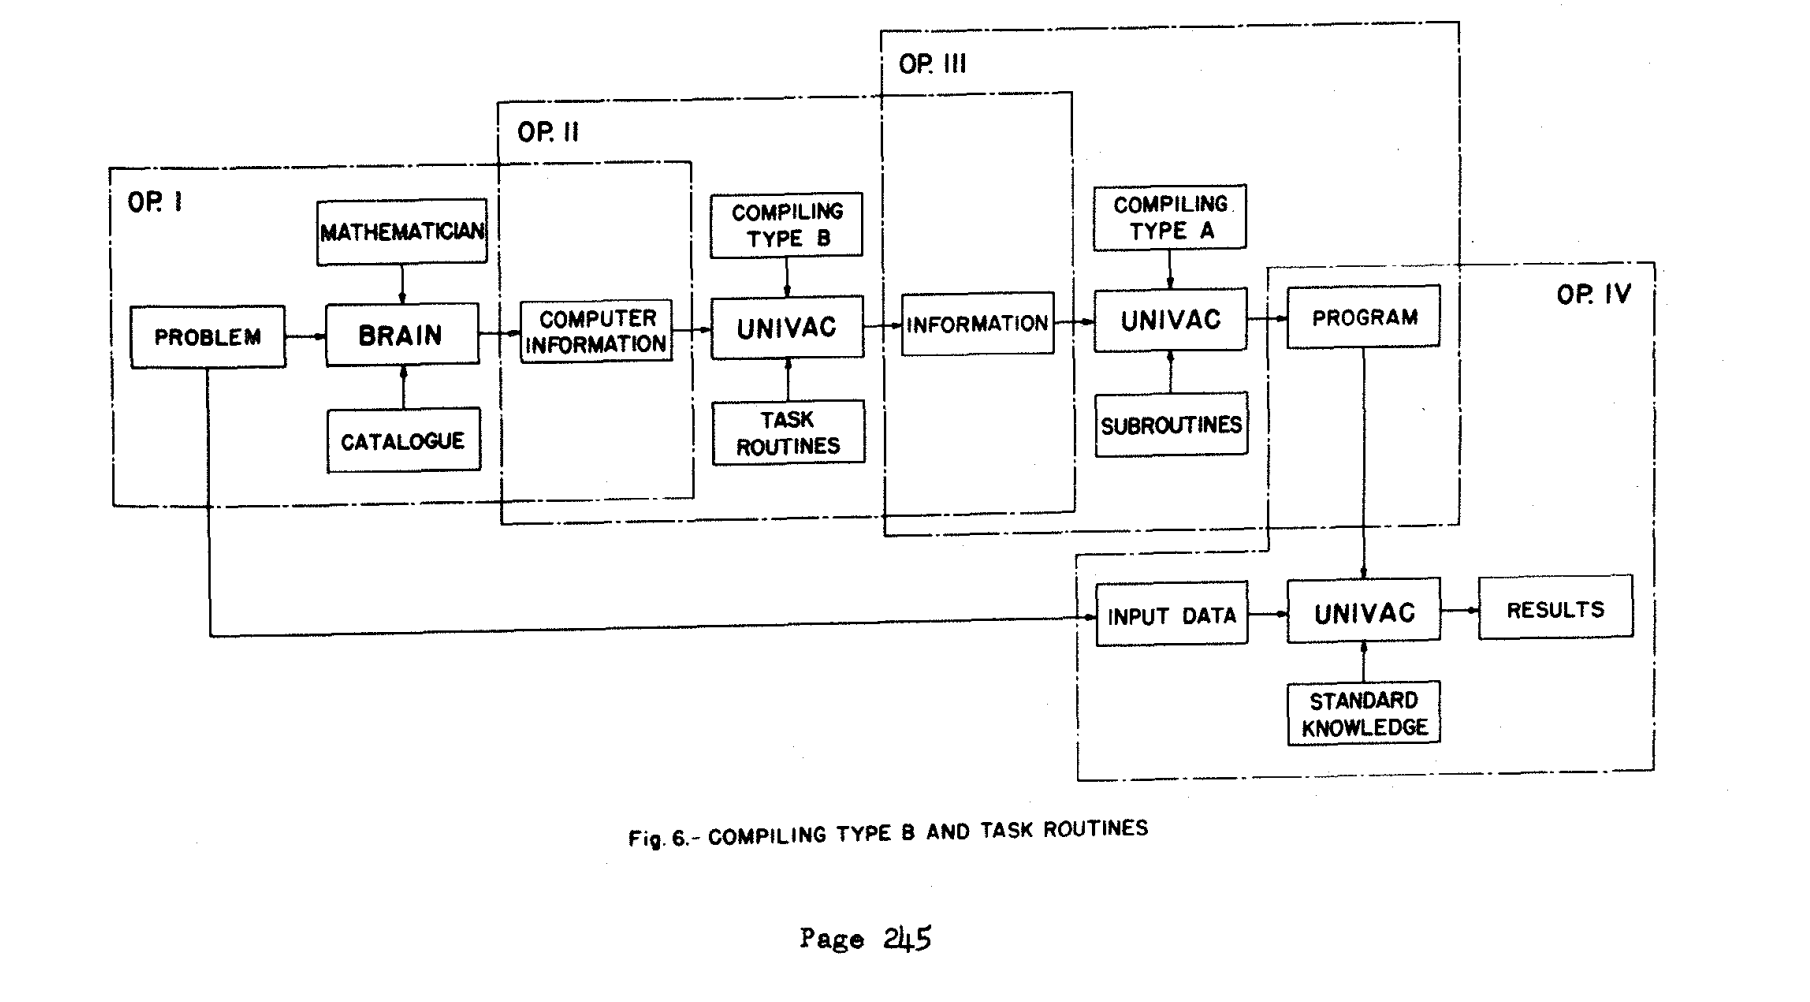
\includegraphics[width=.7\textwidth]{resource/gh_education_of_a_computer_type_fig_6.png}
	\caption{Depiction of \textit{type-B compilation} from Hopper's
		\textit{The Education of a Computer}}
	\label{fig:education-of-a-computer-1952-hopper-f6}
\end{figure}

In this paper, she dubbed her A-0 as a compiler because it was compiling subroutines from a
library into a program, adjusting offsets as necessary. This is far closer to
our modern notion of a linker; its role was to copy machine code from different
locations into a single output program based on an input program \textit{that
	was still mostly in machine code}, save for the references to library
subroutines. Her notion of compilation was perhaps closer to the regular
English meaning of compilation, like that of compiling research papers into a
book. Her hope was that "the programmer may return to being a mathematician,"
though her A-0 did not lift the programmer away from machine code to nearly the
same extent as her subsequent efforts would
\cite{education_of_a_computer_1952_hopper}.
One may also consider this effort
to be the first \textit{standard library}, which would become a major feature
of later compilers and programming languages. This set the stage for compilers
and programming languages providing a default set of useful routines for
programmers to pull from.

The cost of renting a computer remained high relative to the labor cost of
hiring a programmer, thus it was not always economical for computing centers to
use compilers at first. Richard Ridgway and several members of Hopper's team
began testing the A-0 against hand-written programs in the summer of 1952
\cite{ridgway_compiling_routines_1952}. For this study, Richard compared the
computer and labor time spent to calculate a table of values for the equation:

\[
	y = e^{-x^2} \sin\left(\frac{x}{2}\right)
	\quad \text{for } |x| < 1, \Delta x = 0.01.
\]

After an analysis of the same program written by hand and by the A-0, he
concluded that the A-0 (already considered "antique" by 1952, not more than two years
after Hopper began working on it) was cost-efficient to use for most workloads.
Richard writes in \textit{Compiling Routines}\cite{ridgway_compiling_routines_1952}:

\begin{quotation}
	Thus, while more UNIVAC time may be required for the numerical solution of a
	problem as programmed by UNIVAC, more UNIVAC time, \underline{in toto}, is
	consumed by the conventional method. This remains true until the entire problem
	including tis self-contained repetitions is to be repeated, in this case at
	least eighteen times.

	If the total preparation time is considered, the problem must be repeated some
	800 times before the conventional programming method overtakes the compiler
	method. In this case, the compiler used was the "antique," or A-0, the first to
	be constructed and the most inefficient.
\end{quotation}

\subsection{The A-1 and A-2 Compilers}

As Hopper and her team began work on the subsequent A-1 and A-2 compilers,
their motivations shifted away from reducing the tedium of programming to the
economic costs of programming (as is seen in Richard's report).
While computing time was initially far more
costly than human time, as the proportion of computing costs dedicated to human
labor increased over time, the importance of reducing human labor increased as
well.
Her team began working on the A-1 and A-2 in 1953, and the A-2 was
available to UNIVAC customers by the end of the year.
Hopper recruited Herbert Mitchell and Richard Woltman from Aiken's
lab to lead the development of the A-1 and A-2 compilers.
Margaret Harper, Frank Delaney, Mildred Koss, and Richard Ridgway were
the primary developers of these compilers.

There were a number of significant innovations between the A-0 and A-2.
The A-2 performed more of the jobs we associate with compilers today.
Most significantly, by 1954, the A-2 compiler accepted source code
in the form of \textit{pseudocode}, which was a (slightly) more human-friendly
format than plain machine code.
\todo{Some sources reference the A-2 compiler instruction manual,
	but I'm unable to find this source online.}
John Backus described the A-2 compiler's 1954 May update as a significant
improvement because of these pseudocode instructions
\cite{hopl_backus_history_of_fortran}.
He placed the A-2 with Laning and Zierler's algebraic compiler and
his own \FTNI{} compiler as the primary compilers of significance in the
mid 1950s.

Along with pseudocode instructions, this compiler also produced
twelve-character error codes to inform the user why something went wrong
during compilation, which must have been tremendously helpful when users
had been accustomed to the alternative.
The compiler worked in two phases, first constructing an index of the
program and then producing the output machine code, informing the user as
it did so.
The a compiler should be friendly to its users was not necessarily a given at
the time; modern compiler tools owe this to Hopper (to the extend that they
are any better than the A-1).
Another feature of pseudocode instructions is that programs written
in such a manner may be translated to run on different machines, provided
the compiler and standard library are available on those machines.
As far as we know, Hopper never attempted this, however.

By winter of 1953, the A-2 compiler was already being used heavily
by several institutions, including the US Census Bureau and
Lawrence Livermore National Laboratory.
Several of these provided feedback, bug reports, and occasionally features
back to the Remington Rand team.
Nora Moser of the Army Map Service sent Hopper a collection of comiler
improvements, library enhancements, and altogether new libraries in the
winter of 1954.
One cannot overlook the fact that Hopper was a woman in a male dominated
industry, and a number of other women in the industry were her early
collaborators.

Hopper presented on the A-2 at the Pentagon in 1953
\cite{pentagon_hopper_univac_workshop_1953},
facilitating communication with and amongst her users.
This was not the only time she sought to present her team's work
to a wider audience.
Non-UNIVAC customers also expressed interest; more government
agencies and potential customers (with existing IBM machines)
came to learn about their developments.
This open collaboration and sharing of information would set a precedent
for intellectual property in the budding software industry.
She had built the compilers as a way to make programming accessible
and facilitate the sharing of code, and this philosophy extended to
all sorts of information.
She had been successful in a more restricted environment at Harvard,
and she was able to see clearly the merits of a more open industry.

\subsection{After the A-2: A-3, AT-3, MATH-MATIC}

\todo{Should make some mention of interpreters in here.
	Hopper made some observations that might be useful later.}

Not everyone was supportive of the advancements in compiler technology.
There was a significant chunk of the computing industry that thought
programming took too much creativity to be fully automated.
Hopper and John Backus found themselves on the same side of the debate,
both firm in their beliefs that computing should be made accessible.
This is a bit ironic, because IBM would shortly mount a significant effort
towards compilation and competition with Remington Rand, with Backus at the helm.

\begin{quotation}
	Just as freewheeling westerners developed a chauvinistic pride in their
	frontiersmanship and a corresponding conservatism, so many programmers of the
	freewheeling 1950s began to regard themselves as members of a priesthood
	guarding skills and mysteries far too complex for ordinary mortals.
	\cite{Backus_1980_Programming_in_America_in_1950s}
\end{quotation}

Nonetheless, compiler development marched on and the number of compiler
developers continued to grow.
In 1954, Remington Rand formed the Automatic Programming Department
in support of Hopper's team.
With Hopper's ability to teach and communicate along with her compassion
for the programmer, the group thrived.
\todo{Adele Mildred Koss, interview by Kathy Kleiman, 1993,
	talking about how nice it was to work for her.}
Just as Backus was inspired by Laning and Zierler's work at MIT, so too
was Hopper.
In preparation for the Office of Naval Research's 1954 Symposium,
her new department was focused on extending the A-3 compiler,
providing a compiler capable of generating more efficient machine code,
but not much else past what the A-2 could do.
Inspired by the work coming from MIT, they attempted to extend the A-3 to
support source code that resembled equations (more so than the three-address
pseudocode that preceded it, at least).
This new compiler was called the AT-3 and formed one of the two major
components of the MATH-MATIC. The AT-3 was the \textit{Translator}
and the A-3 was the \textit{Arith-Matic Compiler}
\cite{ash_etal_1957_math-matic_manual}.

\begin{figure}[h]
	\centering
	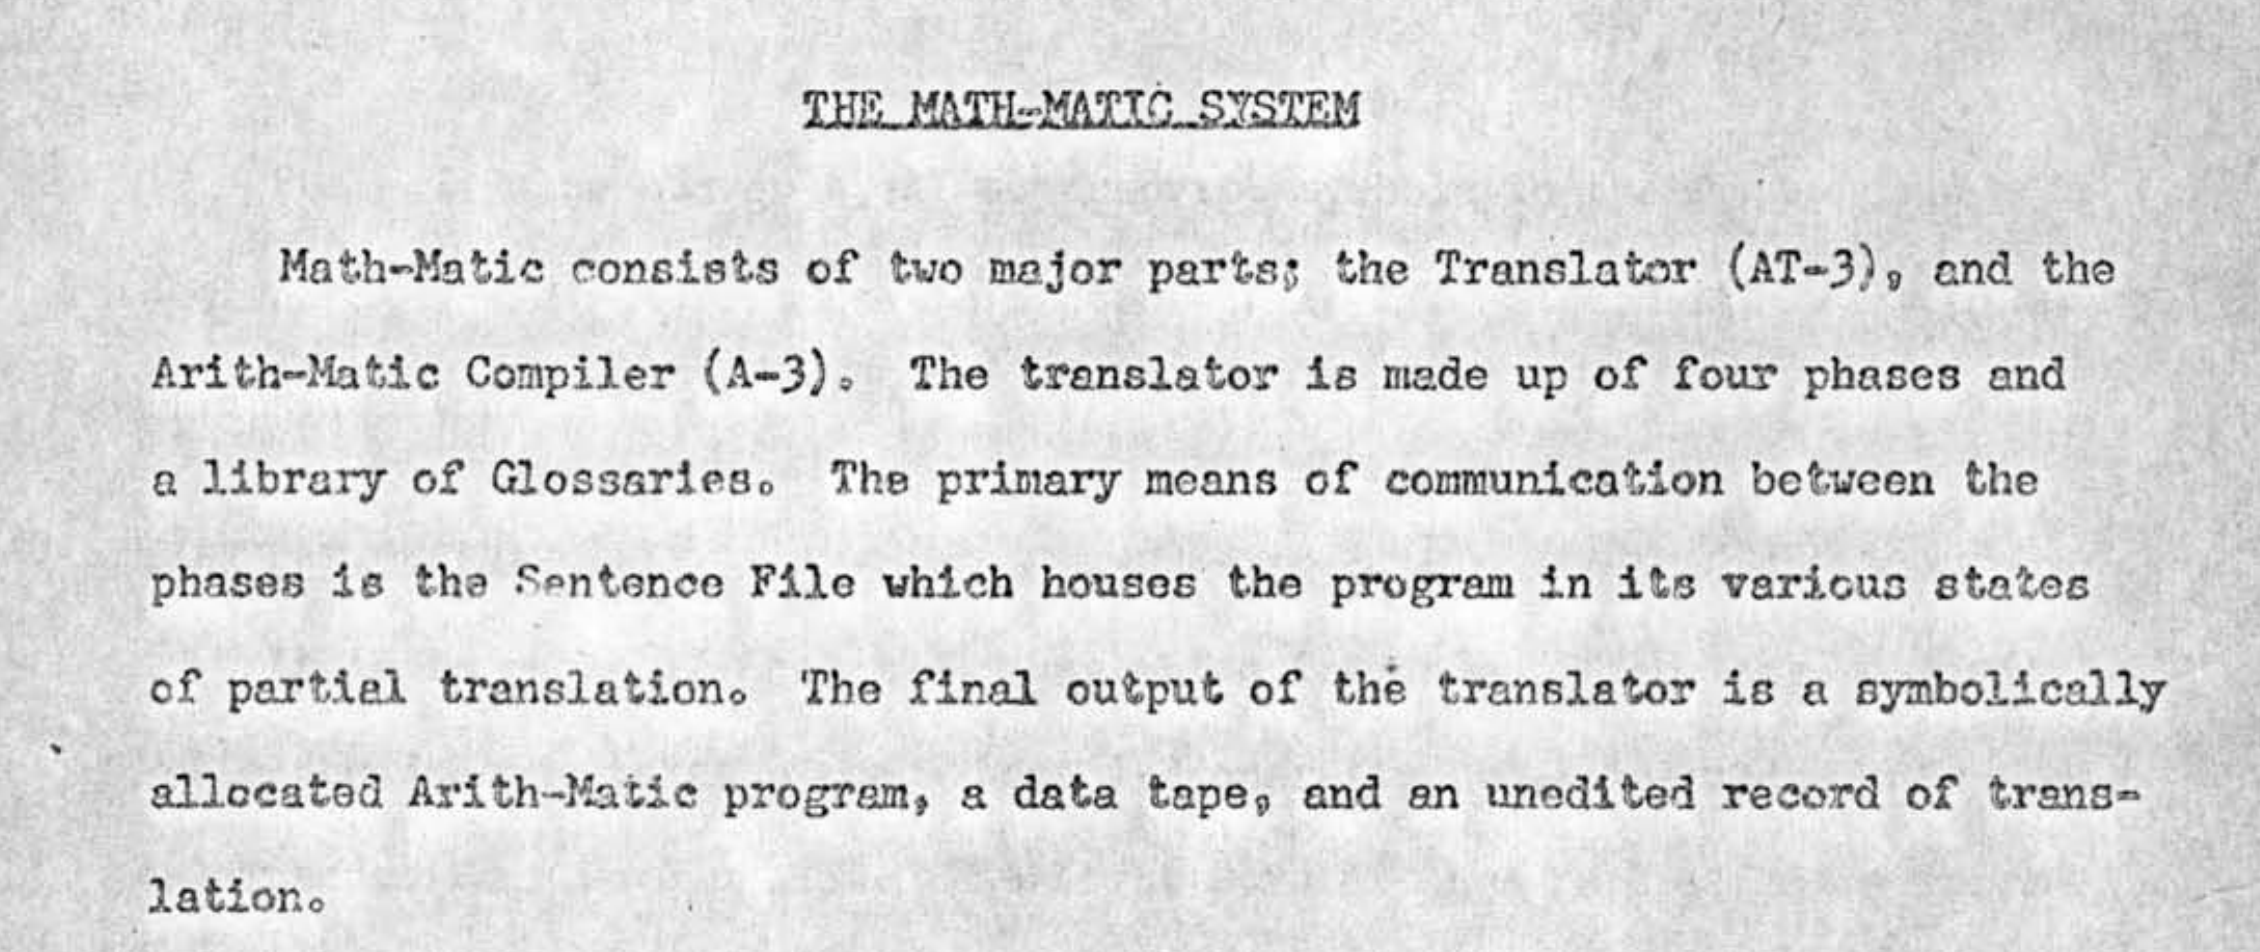
\includegraphics[width=.7\textwidth]{resource/mathmatic-user-guide.png}
	\caption{Excerpt from the MATH-MATIC User's Manual, 1957}
	\label{fig:mathmatic-user-manual}
\end{figure}

It is worth noting that \citetitle{grace_hopper_and_the_invention_of_the_information_age_2009}
\cite{grace_hopper_and_the_invention_of_the_information_age_2009}
appears to have a mistake regarding the A-3 and AT-3:

\begin{quotation}
	Hopper and her colleagues explored the possibility of an
	equation-based programming language, and by 1956 they had
	modified A-3 to the point where it could support a user-friendly
	source code. The resultant AT-3 compiler was later named
	MATH-MATIC.
\end{quotation}

This led me to believe that the A-3 \textit{became} the AT-3 which was
renamed to the MATH-MATIC; however, the MATH-MATIC user manual
\cite{ash_etal_1957_math-matic_manual} specifies that the MATH-MATIC
is composed of the A-3 and the AT-3, which were apparently separate
programs with separate names (the Translator and the Arith-Matic Compiler,
respectively).
See Figure \ref{fig:mathmatic-user-manual}.
Knuth and Pardo describe the MATH-MATIC's development as:
"The language was originally called AT-3; but it received the catchier name
MATH-MATIC in April, 1957, when its preliminary manual was released."
\cite{Knuth_TrabbPardo_1976_Early_Development}
Perhaps the \textit{language} A-3 was extended to become AT-3 which was
renamed MATH-MATIC, while the A-3 and AT-3 compiler programs remained
distinct; because I cannot find sources to clarify this nor the
original programs, I cannot conclusively describe the MATH-MATIC
and its precise relationship to the A-3 and AT-3 past what the
user's manual describes.

Because the MATH-MATIC translated source code into A-3 pseudocode
as an intermediate step, one might also consider this the first compiler
to have an internal intermediate representation.
The MATH-MATIC would last until about 1961, at which point UNIVAC users
were already expecting \FTN{} compilers available on their UNIVAC systems,
favoring IBM's language to Hopper's.

These layers of translation worked against them; the vast majority
of codes at the time were dominated by floating point arithmetic,
so any degradation of floating point performance would be catastrophic for the
overall performance of the system.
Around the same time, John Backus had convinced IBM leadership that
their new machine, the IBM 704, should have index registers and floating point
processing hardware, which is exactly what both UNIVAC and IBM 701 customers
lacked and were spending all their time on.
Now that the 704 accounted for these prior deficiencies in both machines,
Backus's \FTN{} combined with the 704's hardware entirely outclassed the
UNIVAC I and Hopper's MATH-MATIC.

\begin{quotation}
	But the MATH-MATIC programmers did not share the FORTRAN group's enthusiasm for
	efficient machine code; they translated MATH-MATIC source language into A-3 (an
	extension of A-2), and this produced extremely inefficient programs, especially
	considering the fact that arithmetic was all done by floating-point
	subroutines. The UNIVAC computer was no match for an IBM 704 even when it was
	expertly programmed, so MATH-MATIC was of limited utility.

	Knuth and Pardo\cite{Knuth_TrabbPardo_1976_Early_Development}.
\end{quotation}

\subsection{The B-0, FLOW-MATIC, and COBOL}

In an interview for the Computer History Museum's Oral History series,
Hopper explains her motivations for the compilers to follow the A-2
\cite{Hopper_1980_Oral_History}:

\begin{quotation}
	\textbf{Pantages:} At that point did you have a feeling for what was
	happening, in terms of what you were contributing?

	\textbf{Hopper:} No. I've always objected to doing anything over again if I had
	already done it once. That was building the compiler. Then I decided there were
	two kinds of people in the world who were trying to use these things. One was
	people who liked using symbols - mathematicians and people like that. There was
	another bunch of people who were in data processing who hated symbols, and
	wanted words, word-oriented people very definitely. And that was the reason I
	thought we needed two languages.  The data processors did not like symbols,
	abbreviations that didn't convey anything to them.  They were totally
	accustomed to writing things in words. So why not give them a word-oriented
	language? And that was part of what was behind Flow-Matic B-0, which became one
	of the ancestors of COBOL.
\end{quotation}

\begin{figure}
	\centering
	\includegraphics[width=.7\textwidth]{resource/gh_data_processing_compiler.png}
	\caption{Depiction of Hopper's Data Processing Compiler\cite{hopper_1955_preliminary_definitions_data_processing_compiler}}
	\label{fig:data-processing-compiler}
\end{figure}

Hopper's interests in making programming accessible had not waned,
however her target audience shifted.
In January of 1955, she shared a her more radical ideas for a new
compiler in a report titled
\citetitle{hopper_1955_preliminary_definitions_data_processing_compiler}
\cite{hopper_1955_preliminary_definitions_data_processing_compiler}
.
This compiler would take on several names: first, the data-processing
compiler as outlined in the 1955 paper, then the B-0, the Procedure Translator,
and finally the FLOW-MATIC.

\begin{quotation}
	This was what she originally called the data processing compiler in January,
	1955; it was soon to be known as "B-0," later as the "Procedure
	Translator", and finally as FLOW-MATIC, This language used English
	words, somewhat as MATH-MATIC did but more so, and its operations concentrated
	on business applications.
	\cite{history_of_computing_in_the_twentieth_century_1980}
\end{quotation}

\begin{figure}[h]
	\centering
	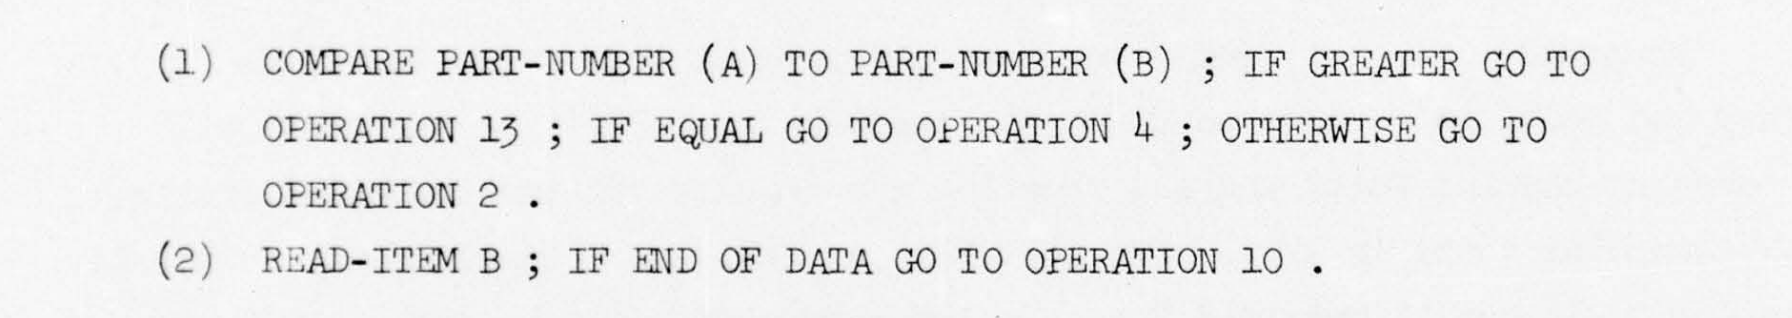
\includegraphics[width=.7\textwidth]{resource/flow-matic-example-knuth-pardo.png}
	\caption{Example FLOW-MATIC code from Knuth and Trabb Pardo\cite{Knuth_TrabbPardo_1976_Early_Development}}
	\label{fig:knuth-pardo-flow-matic-example}
\end{figure}

Always concerned with how intelligible her users would find her compilers
and programming languages, she focused more on business applications and managers.
Donald Knuth and Luis Trabb Pardo describe the FLOW-MATIC as
"far more influential and successful, since it broke important new ground."
\cite{Knuth_TrabbPardo_1976_Early_Development}
(see also Figure \ref{fig:knuth-pardo-flow-matic-example}).
Instead of catering her compilers to mathematicians and scientists
by introducing mathematical symbols and notation, she sent members of
her team to UNIVAC customers to learn about their \textit{business} needs.

\begin{figure}
	\centering
	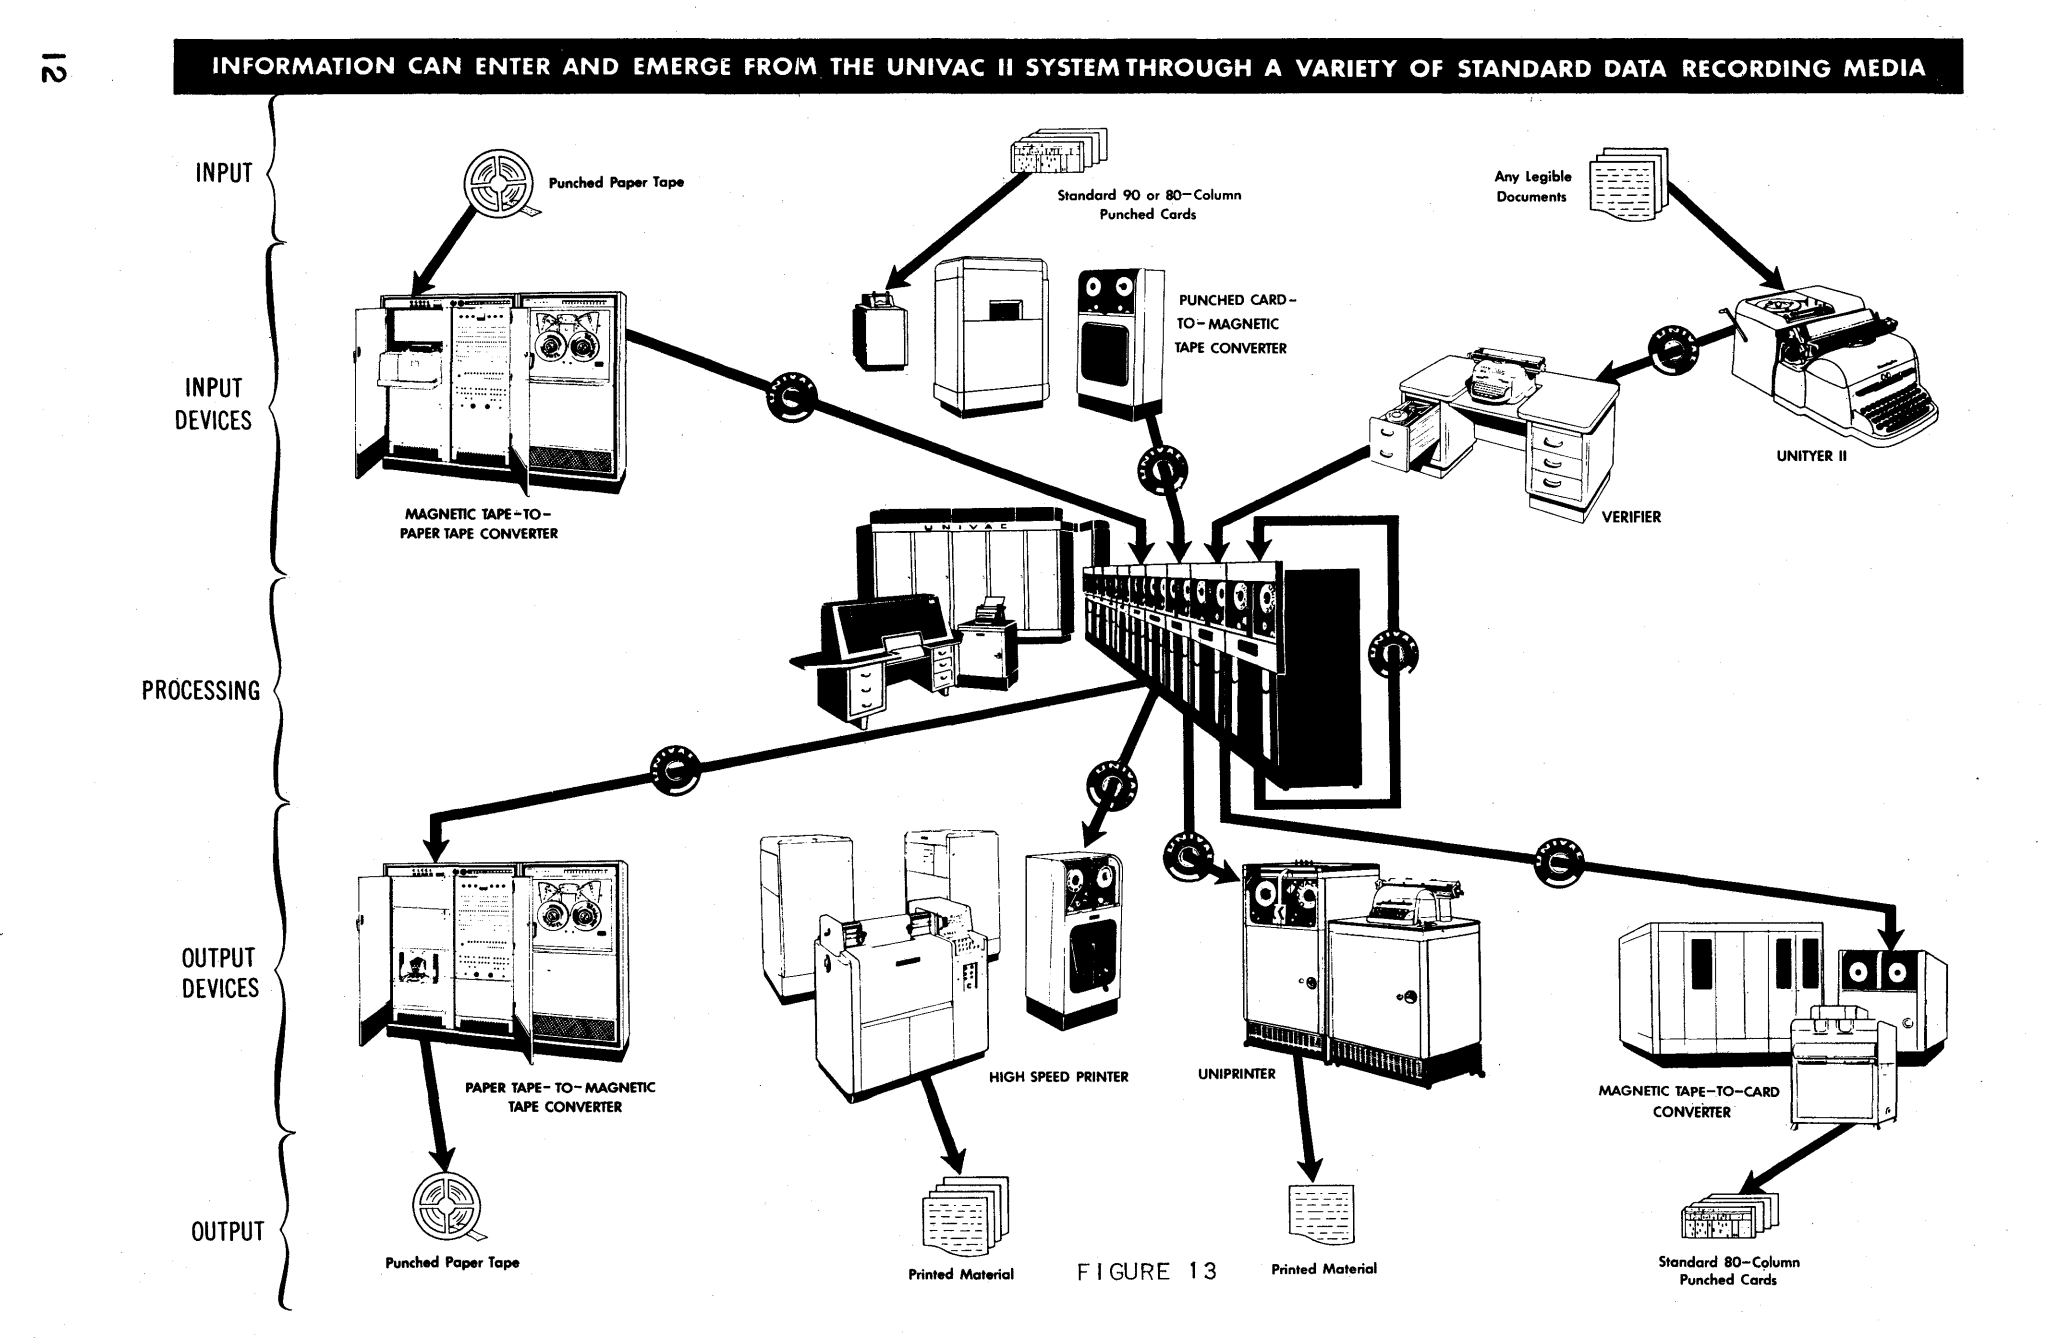
\includegraphics[width=.7\textwidth]{resource/flow-matic-ad-1959.png}
	\caption{Advertisement for FLOW-MATIC and UNIVAC II}
	\label{fig:flow-matic-ad-1959}
\end{figure}

The business compiler B-0 was first made available to UNIVAC customers
at the start of 1958.
Shortly thereafter, Remington Rand merged with Sperry Gyroscope to form Sperry Rand.
The marketing department of the newly formed company renamed the B-0
to FLOW-MATIC.
Catering to business users, the FLOW-MATIC was programmed in English-like
statements such as:
\texttt{IF EQUAL GO TO OPERATION 5 ; OTHERWISE GO TO OPERATION 2 .}
The group toyed with using abbreviations for common words, but
after studying their customer's programs, they found that too many
abbreviations could be mapped to different words based on the customer,
so the abbreviated form was abandoned.
Jean Sammet notes: "A preliminary manual
for the running system was marked Company Confidential and dated July,
1957; it was available to me at that time since I was an employee of the
Sperry Rand Corporation"
\cite{sammet_programming_languages_history_and_fundamentals_1969}.
The first generally available version of this document was available
in early 1958 in \citetitle{sperryrand_1959_flowmatic}\cite{sperryrand_1959_flowmatic}.
In this manual, one now finds advertisements for the UNIVAC II\ref{fig:flow-matic-ad-1959}.

In this document, one also finds a crude method for specifying the language,
which the reader should note; Backus would propose a more formal method
for specifying programming languages not long after this.
For example, the \texttt{CLOSE-OUT} command is specified in the FLOW-MATIC manual as
\footnote{The $\Delta$ symbols were present in the original manual because it signified
	an empty space in the punchcards the FLOW-MATIC was written on}:

\[
	\Delta \text{\texttt{CLOSE-OUT}} \Delta
	\left[
		\begin{array}{c}
			\text{file} \\
			\text{files}
		\end{array}
		\right]
	\Delta
	f_1
	\Delta
	\left[
		f_2
		\Delta
		f_3
		\Delta
		\dots
		\Delta
		f_n
		\right]
\]

There was no format method for specifying languages at the time.
In 1959, one of the B-0 developers, Mary Hawes, contacted Sperry Rand about a meeting to
discuss the direction of compilers for business applications.
\todo{In some places, Hawes is described as one of the B-0 developers which leads
	me to believe she worked at RR or SR, but Sammet points out that she worked
	for the ElectroData division of the Burroughs Corporation. Need to clarify.}
Sammet states\cite{sammet_early_history_of_cobol_1978} that Block's 1959
\textit{Report on Meeting held at University of Pennsylvania Computing Center} names
Hawes as having called this meeting:

\begin{quotation}
	\dots meeting was the result of a request by
	Mary K. Hawes (ElectroData Division, Burroughs Corporation) to plan a formal meeting
	involving both users and manufacturers where plans could be prepared to develop the
	specifications for a common business language for automatic digital computers.
\end{quotation}

I am unable to retrieve this document; we will take Jean Sammet's word for it.
\todo{there is not much about Mary Hawes available online,
	I can't even find the papers Hawes originally wrote.
	Try to find \textit{Mary Hawes, “Automatic Routines for Commercial Installations”}}
Through a connection at the Department of Defense (Charles Phillips), this group
asked the DoD to sponsor the meetings and recommended a list of attendees, including
7 representatives from computer manufacturers and 14 from user organizations.
In an ACM talk on September 1, 1959, Phillips remarked that "embarrassed that
the idea for such a common language had not had its origin by that time in
Defense since we would benefit so greatly from the success of such a project."
\cite[Phillips, as quoted by Sammet in]{sammet_programming_languages_history_and_fundamentals_1969}.
There was a great deal of discussion around a common business language
that could be shared across different computer systems and reduce the overall cost of programming.
\textit{Three separate committees} were formed for this purpose; a short, medium, and long-term committee.
Sammet remarks that "the importance of the notion of Short and
Intermediate-Range Committees is absolutely crucial to an understanding of the
development of COBOL"\cite{sammet_early_history_of_cobol_1978}.
She went on to say:

\begin{quotation}
	This wording is clearly ambiguous, and at the time, there was some discussion
	as to whether or not we were to try and create a language. It was by no means
	clear \textit{then} that we were to do anything \textit{except} try and
	\textit{combine} the three known languages of the time.
	These were FLOW-MATIC, \dots AIMACO, \dots and COMTRAN
\end{quotation}

AIMACO was a language developed at the Air Force, and COMTRAN (renamed to Commercial Translator)
existed only in an IBM manual whose implementation had never even started.
Clearly, Hopper and Sperry Rand's FLOW-MATIC was the most mature of these languages.
Indeed, Hopper pointed out that the language resulting from these committees
was almost entirely FLOW-MATIC\cite{Hopper_1980_Oral_History}, though the committee notes
did not say as much. Hopper's lack of an ego and her diplomatic skills
led her to give credit liberally in order to drive consensus.

\begin{quotation}
	We'd written FLOW-MATIC before that, and if you take the FLOW-MATIC
	manual and compare it with COBOL 60 you'll find COBOL 60 is 95\% FLOW-MATIC. So the
	influence of Commercial Translator in fact was extremely small. But I figured the thing to do was
	corral those people and when we had something to say, we'd say it was a compound of FLOW-MATIC
	and Commercial Translator and keep the other people happy and wouldn't try to knock
	us out. We'd give them some credit and they'd have to get on board with us. But if you compare
	the two manuals you'd find that it had hardly any influence at all. But if you gave them credit for
	it, why they'd go right along with you. If you didn't, they'd fight you. You can always give credit,
	you can always afford to.

	That again is the practical. Think about the other guy and his position and his interest. You are
	always trying to work with people rather than against them. You've got a new idea; give the
	boss credit for it. It doesn't cost you anything.
\end{quotation}

Here the reader should note Sammet's observation of the differing goals of the three committees:

\begin{quotation}
	I am certainly convinced in my own mind that had the Short-Range Committee
	realized at the outset that the language it created (i.e., COBOL) was going to
	be in use for such a long period of time, it would have gone about the task
	quite differently and produced a rather different result. But I believe that
	most of us viewed our work as a stopgap measure--a very important stopgap
	indeed, but not something intended for longevity.
\end{quotation}

Most of the disdain for COBOL may indeed come from the fact that it was designed by the \textit{short term}
committee, which was solely trying to combine the existing compiler and programming language practices
of the time into one language to prevent further bifurcation.
If COBOL seems like a mishmash of different ideas designed by committee without proper
foresight or thoughtful design, well, it more or less was.
Yet another committee was formed on top of these three, the "Committee on Data Systems Languages"
or CODASYL, which would be the exeucutive committee steering the direction of the other three.

\subsection{COBOL Comes Into Focus}

Throughout September and October of 1959, the short-term committee met
regularly to build consensus around this new language.
There were a number of similar names considered before settling on COBOL:

\[
	\begin{array}{ll}
		\text{BUSY}    & \text{Business System}                  \\
		\text{BUSYL}   & \text{Business System Language}         \\
		\text{INFOSYL} & \text{Information System Language}      \\
		\text{DATASYL} & \text{Data System Language}             \\
		\text{COSYL}   & \text{Common Systems Language}          \\
		\text{COCOSYL} & \text{Common Computer Systems Language} \\
	\end{array}
\]

On September 18th of that year, the committee settled on
COBOL, according to Jean Sammet's personal notes\cite{sammet_early_history_of_cobol_1978}.
I spare the reader of the full details of the committee's meetings,
and encourage interested readers to consult Sammet's detailed notes on the proceedings.
Perhaps the most important conclusion from these meetings was that there existed a
\textit{Basic COBOL}, and that no computer manufacturer could claim to support COBOL
unless they supported this core subset of the language.
This set the stage for numerous modern programming languages that contain a
standard language specification that all compilers must support to claim to
be a compiler for that language, key examples being C and C++.

The first correct and complete compilation of a COBOL program was performed in
August of 1960 on an RCA 501.
In December of that year Sperry Rand and RCA each wrote COBOL programs,
ran them on their own machines, exchanged programs, and verified that they ran on
the other manufacturer's machine as well (a UNIVAC II and an RCA 501).
Thus was the first programming language standardized to the point that different compilers
running on different machines could compile the same program correctly.

While Hopper's legacy tends to be tied to COBOL, I believe her true legacy lies in
her passion for open collaboration and making programming accessible.
She thought deeply about the needs of her users; she sent employees to study them
and learn what their pain points were and how best the compiler developers could serve them.
She considered how to tailor her technology to her users, how to make her compilers
more friendly speakers of other languages, and how to make compilers produce understandable
error message and make them more debuggable.
She facilitated communication between users and developers and advocated for
a liberal notion of intellectual property to facilitate the sharing of ideas and programs;
this outlook would lead to a cambrian explosion of compiler technology in the open-source era
decades after her work on COBOL.
This is where I think Grace Hopper's true legacy lies, not solely in the language
cobbled together by a potpourri of committees with a short-term view.
